\documentclass[10pt]{article}
\usepackage{graphicx}
\usepackage{amssymb}
\usepackage[fleqn]{amsmath}
\usepackage{nccmath}
\usepackage{cases}
\usepackage{hyperref}
\usepackage{multicol}
\usepackage{tikz}
\usepackage{pgfplots}
\usepackage{enumitem}
\usepackage{pdfpages}
\pgfplotsset{compat=1.18}
\usepackage{float}


\title{\bf Math 151b: Problem Set 8}
\author{\bf Owen Jones}
\begin{document}
\maketitle
\section*{Problem 1:}
\begin{enumerate}[label=(\alph*)]
    \item Taking the $\log$ of both sides $\log(y)=\log(\alpha)-\beta x$.\\
    Let $\mathbf{A}=\begin{bmatrix}
        x_1 & 1\\
        x_2 & 1\\
        \vdots & \vdots\\
        x_m & 1
    \end{bmatrix}$, $\mathbf{x}=\begin{bmatrix}
        -\beta\\
        \log(\alpha)
    \end{bmatrix}$, and $\mathbf{b}=\begin{bmatrix}
        \log(y_1)\\
        \log(y_2)\\
        \vdots\\
        \log(y_m)
    \end{bmatrix}$
    \item Let $\overline{X}=\frac{1}{m}\sum_{i=1}^{m}x_i$, $\overline{X^2}=\frac{1}{m}\sum_{i=1}^{m}x_i^2$, $\overline{\log(Y)}=\frac{1}{m}\sum_{i=1}^{m}\log(y_i)$, $\overline{X\log(Y)}=\frac{1}{m}\sum_{i=1}^{m}x_i\log(y_i)$.
    \begin{align*}
        &\mathbf{x}^*={(\mathbf{A}^\top\mathbf{A})}^{-1}\mathbf{A}^\top\mathbf{b}\\
        &=\begin{bmatrix}
            m\overline{X^2} & m\overline{X}\\
            m\overline{X} & m
        \end{bmatrix}^{-1}
        \begin{bmatrix}
            m\overline{X\log(Y)}\\
            m\overline{\log(Y)}
        \end{bmatrix}=\begin{bmatrix}
            \overline{X^2} & \overline{X}\\
            \overline{X} & 1
        \end{bmatrix}^{-1}
        \begin{bmatrix}
            \overline{X\log(Y)}\\
            \overline{\log(Y)}
        \end{bmatrix}\\
        &=\frac{1}{\overline{X^2}-\overline{X}^2}
        \begin{bmatrix}
            1 & -\overline{X}\\
            -\overline{X} & \overline{X^2}
        \end{bmatrix}
        \begin{bmatrix}
            \overline{X\log(Y)}\\
            \overline{\log(Y)}
        \end{bmatrix}\\
        &=\frac{1}{\overline{X^2}-\overline{X}^2}\begin{bmatrix}
            \overline{X\log(Y)}-\overline{X}\cdot\overline{\log(Y)}\\
            \overline{X^2}\cdot\overline{\log(Y)}-\overline{X}\cdot\overline{X\log(Y)}
        \end{bmatrix}\\
        &\Rightarrow \beta=\frac{\overline{X}\cdot\overline{\log(Y)}-\overline{X\log(Y)}}{\overline{X^2}-\overline{X}^2},\alpha=\exp(\frac{\overline{X^2}\cdot\overline{\log(Y)}-\overline{X}\cdot\overline{X\log(Y)}}{\overline{X^2}-\overline{X}^2})
    \end{align*}
\end{enumerate}
\section*{Problem 2:}
\begin{enumerate}[label=(\alph*)]
    \item $(P_\mathbf{q})^2=(\mathbf{q}\mathbf{q}^\top)(\mathbf{q}\mathbf{q}^\top)=\mathbf{q}(\mathbf{q}^\top\mathbf{q})\mathbf{q}^\top=\mathbf{q}{\lVert\mathbf{q}\rVert}^2\mathbf{q}^\top=\mathbf{q}\mathbf{q}^\top=P_\mathbf{q}$ because $\mathbf{q}$ is a unit vector. $P_\mathbf{q}^\top={(\mathbf{q}\mathbf{q}^\top)}^\top={(\mathbf{q}^\top)}^\top{(\mathbf{q})}^\top=\mathbf{q}\mathbf{q}^\top=P_\mathbf{q}$. By transitivity, $P_\mathbf{q}^\top={(P_\mathbf{q})}^2$
    \item ${(I-P)}^2=I^2-2IP+P^2=I-2P+P=I-P$ because if $P$ is an orthogonal projector, then $P^2=P$. ${(I-P)}^\top=I^\top-P^\top=I-P$ because if $P$ is an orthogonal projector, then $P^\top=P$. Thus, $I-P$ is an orthogonal projector.\\
    Since $P$ is an orthogonal projector onto $W$, $P\mathbf{v}\in W$ and $\mathbf{v}-P\mathbf{v}\in W^\perp$ for all $\mathbf{v}\in\mathbb{R}^m$. Thus, $(I-P)\mathbf{v}=\mathbf{v}-P\mathbf{v}\in W^\perp$, so $(I-P)$ is an orthogonal projector onto $W^\perp$. We showed in part (a) that $P_\mathbf{q}$ is an orthogonal projector onto $span\{\mathbf{q}\}$, so by what we showed earlier in part (b), $I-P_\mathbf{q}$ must be an orthogonal projector onto $span\{\mathbf{q}\}^\perp$.
\end{enumerate}
\section*{Problem 3:}
\begin{enumerate}[label=(\alph*)]
    \item Proof by induction:\\
    Base Case: 
    \begin{align*}
        &P_{\perp \mathbf{q}_2}P_{\perp \mathbf{q}_1}=(I-\mathbf{q}_2\mathbf{q}_2^\top)(I-\mathbf{q}_1\mathbf{q}_1^\top)\\
        &=I^2-\mathbf{q}_2\mathbf{q}_2^\top-\mathbf{q}_1\mathbf{q}_1^\top+\mathbf{q}_2(\mathbf{q}_2^\top\mathbf{q}_1)\mathbf{q}_1^\top\\
        &=I-\mathbf{q}_2\mathbf{q}_2^\top-\mathbf{q}_1\mathbf{q}_1^\top
    \end{align*}
    $\mathbf{q}_2^\top\mathbf{q}_1=0$ because $\{\mathbf{q}_1,\mathbf{q}_2,\ldots,\mathbf{q}_n\}$ is an orthonormal set.\\
    Induction hypothesis: Assume for some $2\le k< n$ 
    \begin{align*}
        &P_{\perp \mathbf{q}_k}\ldots P_{\perp \mathbf{q}_2}P_{\perp \mathbf{q}_1}=I-\mathbf{q}_k\mathbf{q}_k^\top-\cdots-\mathbf{q}_2\mathbf{q}_2^\top-\mathbf{q}_1\mathbf{q}_1^\top
    \end{align*}
    Induction step:
    \begin{align*}
       &P_{\perp \mathbf{q}_{k+1}}P_{\perp \mathbf{q}_k}\ldots P_{\perp \mathbf{q}_2}P_{\perp \mathbf{q}_1}=(I-\mathbf{q}_{k+1}\mathbf{q}_{k+1}^\top)(I-\mathbf{q}_k\mathbf{q}_k^\top-\cdots-\mathbf{q}_2\mathbf{q}_2^\top-\mathbf{q}_1\mathbf{q}_1^\top)\\
       &=I-\mathbf{q}_k\mathbf{q}_k^\top-\cdots-\mathbf{q}_2\mathbf{q}_2^\top-\mathbf{q}_1\mathbf{q}_1^\top-\mathbf{q}_{k+1}\mathbf{q}_{k+1}^\top\\
       &+\mathbf{q}_{k+1}(\mathbf{q}_{k+1}^\top\mathbf{q}_k)\mathbf{q}_k^\top+\cdots+\mathbf{q}_{k+1}(\mathbf{q}_{k+1}^\top\mathbf{q}_2)\mathbf{q}_2^\top+\mathbf{q}_{k+1}(\mathbf{q}_{k+1}^\top\mathbf{q}_1)\mathbf{q}_1^\top\\
       &=I-\mathbf{q}_{k+1}\mathbf{q}_{k+1}^\top-\mathbf{q}_k\mathbf{q}_k^\top-\cdots-\mathbf{q}_2\mathbf{q}_2^\top-\mathbf{q}_1\mathbf{q}_1^\top
    \end{align*}
    $\mathbf{q}_{k+1}^\top\mathbf{q}_i=0$ for all $i=1\ldots k$ because $\{\mathbf{q}_1,\mathbf{q}_2,\ldots,\mathbf{q}_n\}$ is an orthonormal set.\\
    Hence, by induction, $P_{\perp \mathbf{q}_k}\ldots P_{\perp \mathbf{q}_2}P_{\perp \mathbf{q}_1}=I-\mathbf{q}_k\mathbf{q}_k^\top-\cdots-\mathbf{q}_2\mathbf{q}_2^\top-\mathbf{q}_1\mathbf{q}_1^\top$ for all $2\le k\le n$.
    \item If we change the order we apply the orthogonal projectors, we simply change the order of the linear combination of $\mathbf{q}_i\mathbf{q}_i^\top$s. However, addition and subtraction are commutative, so this would not change $P_{\perp \mathbf{q}_k}\ldots P_{\perp \mathbf{q}_2}P_{\perp \mathbf{q}_1}$.
    Thus, $P_{\perp W}=P_{\perp \mathbf{q}_k}\ldots P_{\perp \mathbf{q}_2}P_{\perp \mathbf{q}_1}$ for any permutation of $\{\mathbf{q}_1,\mathbf{q}_2,\ldots,\mathbf{q}_n\}$.
\end{enumerate}
\section*{Problem 4:}
\begin{enumerate}[label=(\alph*)]
    \item Suppose we have a collection of data points in a vertical line i.e, they all have the same $x$ coordinate but different $y$ coordinates $y_1,y_2\ldots y_m$.\\
    Let $\mathbf{A}=\begin{bmatrix}
        1 & x\\
        1 & x\\
        \vdots & \vdots\\
        1 & x
    \end{bmatrix}$, $\mathbf{x}=\begin{bmatrix}
        c_0\\
        c_1
    \end{bmatrix}$, and $ \mathbf{b}=\begin{bmatrix}
        y_1\\
        y_2\\
        \vdots\\
        y_m
    \end{bmatrix}$. $\mathbf{b}\not\in span\{\begin{bmatrix}
        1\\
        1\\
        \vdots\\
        1
    \end{bmatrix}\}\Rightarrow \mathbf{b}\not\in \mathcal{R}(\mathbf{A})$.\\
    $\mathbf{A}^\top\mathbf{A}=\begin{bmatrix}
        m & mx\\
        mx & mx^2
    \end{bmatrix}$ is not invertible because the columns are linearly dependent, so there are multiple least square solutions.\\
    $\begin{bmatrix}
        m & mx\\
        mx & mx^2
    \end{bmatrix}
    \begin{bmatrix}
        c_0\\
        c_1
    \end{bmatrix}=
    \begin{bmatrix}
        \sum_{i=1}^{m}y_i\\
        x\sum_{i=1}^{m}y_i
    \end{bmatrix}$\\
    $\begin{bmatrix}
        1\\
        x
    \end{bmatrix}(c_0m+c_1mx)=\begin{bmatrix}
        1\\
        x
    \end{bmatrix}\sum_{i=1}^{m}y_i$\\
    so any $c_0,c_1$ that satisfies $c_0+c_1x=\frac{1}{m}\sum_{i=1}^{m}y_i$ will be a least square solution.
    \item Let $a_1,a_2,\ldots, a_n$ denote the columns of $A$. 
    $a_i=Q r_i$ where $r_i$ is the $i^{th}$ column of $R$.
    It follows $\alpha_1 a_1+\alpha_2 a_2+\cdots+\alpha_n a_n=Q(\alpha_1 r_1+\alpha_2 r_2+\cdots+\alpha_n r_n)$.
    $Q$ is an orthogonal matrix, so it has rank $n$. Thus, $Q(\alpha_1 r_1+\alpha_2 r_2+\cdots+\alpha_n r_n)=0$ iff $\alpha_1 r_1+\alpha_2 r_2+\cdots+\alpha_n r_n=0$.\\
    If $A$ has full rank, then $\alpha_1 a_1+\alpha_2 a_2+\cdots+\alpha_n a_n=0$ iff $\alpha_i=0$ for $i=1\ldots n$.
    This implies $\alpha_1 r_1+\alpha_2 r_2+\cdots+\alpha_n r_n=0$ iff $\alpha_i=0$ for $i=1\ldots n$.
    Thus, the columns of $R$ are linearly independent. Since $R$ is upper triangular, this is only true when the product of the diagonal is nonzero. Thus, all the entries of the diagonal are nonzero.\\
    If all the diagonal entries of $R$ are nonzero, the its columns are linearly independent. 
    Thus, $Q(\alpha_1 r_1+\alpha_2 r_2+\cdots+\alpha_n r_n)=0$ iff $\alpha_i=0$ for $i=1\ldots n$.
    This implies $\alpha_1 a_1+\alpha_2 a_2+\cdots+\alpha_n a_n=0$ iff $\alpha_i=0$ for $i=1\ldots n$ because $a_i=Qr_i$.
    Since the columns of $A$ are linearly independent, $A$ has full rank.
\end{enumerate}
\section*{Problem 5:}
\begin{enumerate}[label=(\alph*)]
    \item \begin{enumerate}[label=(\roman*)]
        \item Condition number for overdetermined system: $230733.08869696865$\\
        Condition number for normal equation: $53237758117.525375$\\
        $cond(A)=\sqrt{cond(A^\top A)}$
        \item $c_0=-4.88868679\times 10^6$, $c_1=2.58447429\times 10^3$
        \begin{figure}[H]
            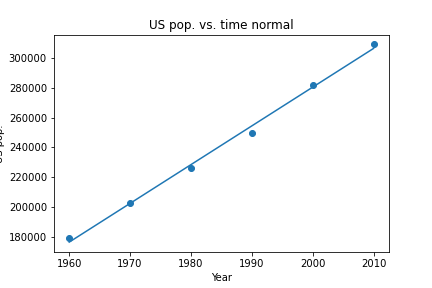
\includegraphics[scale=0.5]{US pop vs time normal.png}
        \end{figure}
        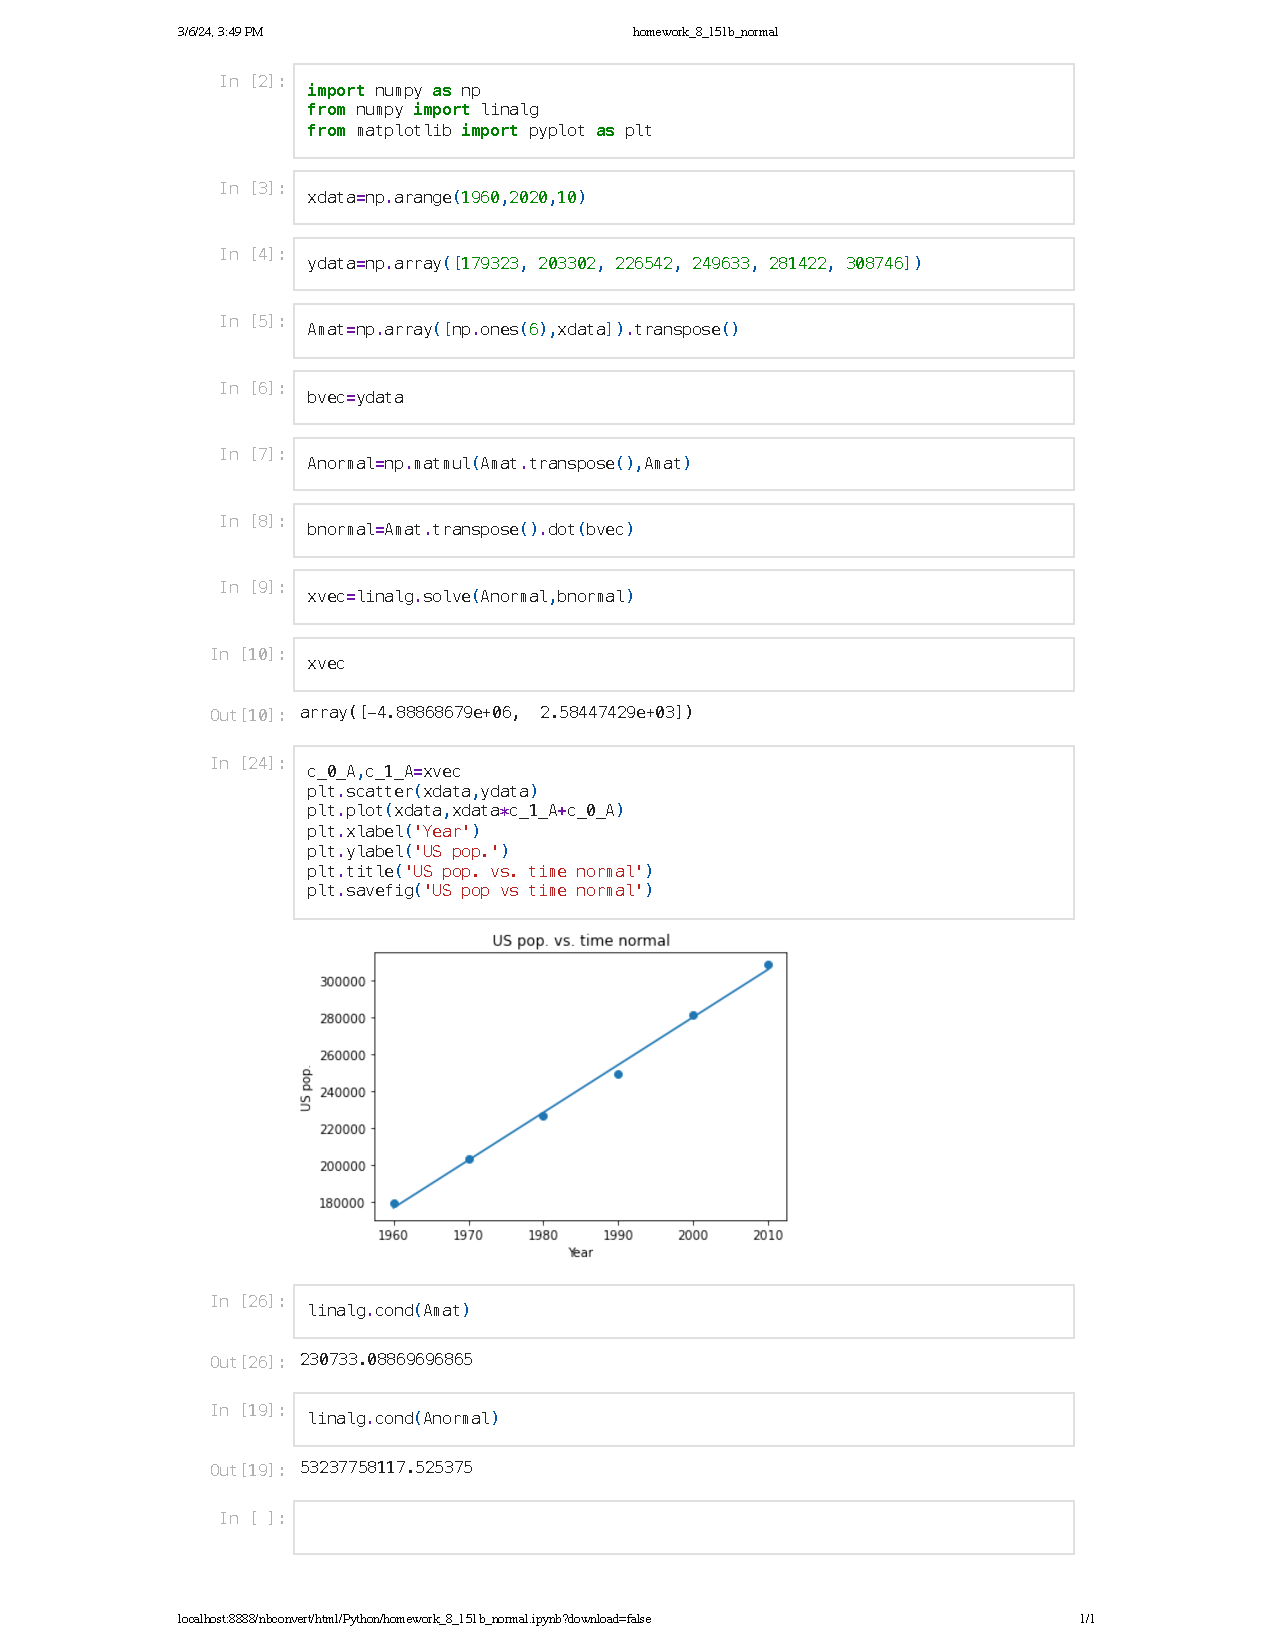
\includepdf{homework_8_151b_normal.pdf}
    \end{enumerate}
    \item Condition number for QR: $230733.08869696865$
    \begin{figure}[H]
        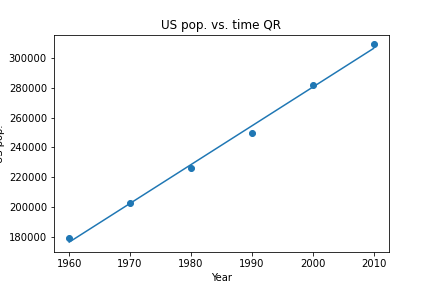
\includegraphics[scale=0.5]{US pop vs time QR.png}
    \end{figure}
    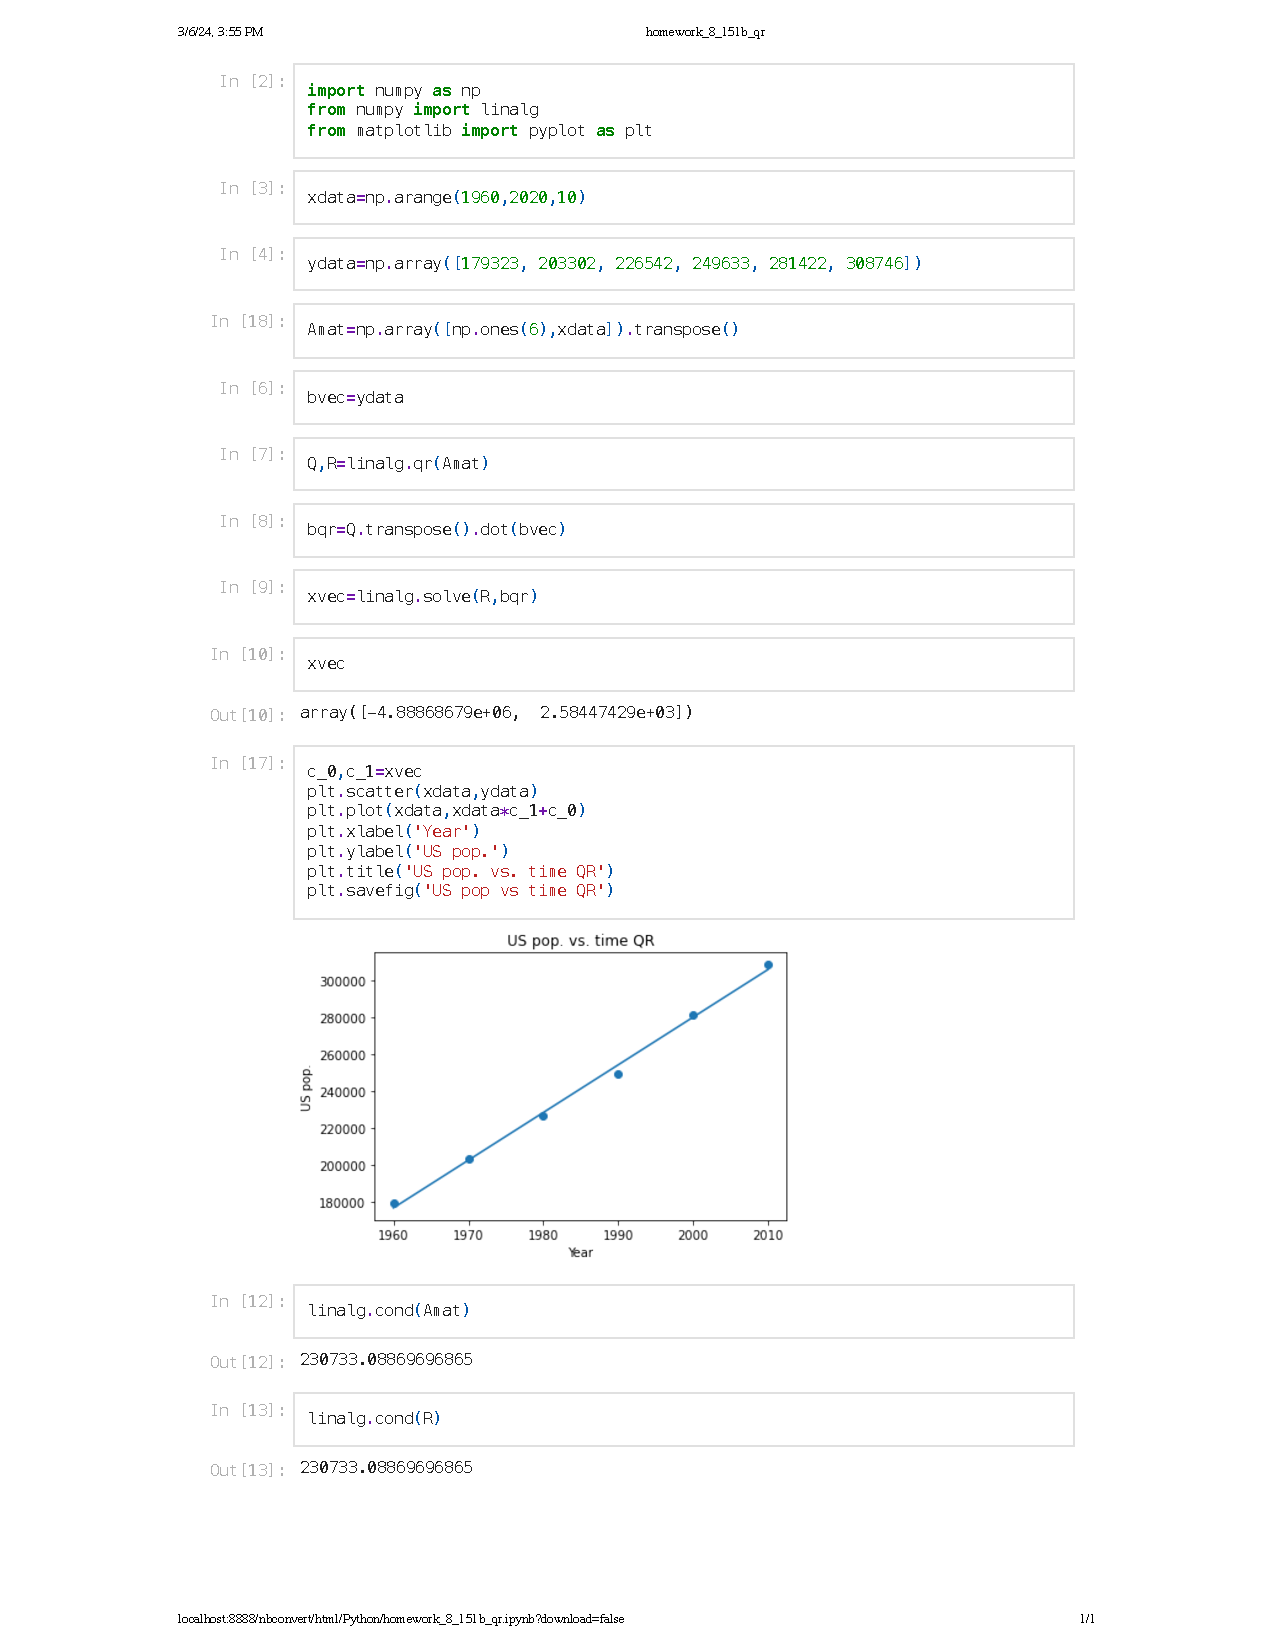
\includepdf{homework_8_151b_qr.pdf}
    \item \begin{enumerate}
        \item Condition number for overdetermined system: $62250894343.79537$\\
        Condition number for normal equation: $8.00160109303428\times 10^{21}$\\
        \item Condition number for QR: $62250894343.79537$\\
        \item Condition number for recentered data QR method: $2843.8719526832056$
    \end{enumerate}
\end{enumerate}
\end{document}